\chapter{Continuous Integration}
Continuous Integration is geregeld door TravisCI, voor open source projecten is TravisCI gratis te gebruiken.
Omdat het project met Gradle is gebouwd is het makkelijk om CI ondersteuning toe te voegen aan de backend.
Het commando "gradle test" draait alle tests in het project, als er iets fout gaat is dit ook meteen in Github zichtbaar.

\begin{figure}[H]
	\includegraphics[width=\textwidth]{images/TravisCi.png}
	\caption{Overzicht TravisCI}
	\label{fig:travisci-commits}
\end{figure}
Travis CI kan geconfigureerd worden met een bestand dat .travis.yml heet, dit bestand is zoals te zien in .yml formaat.
Dit bestand moet in de root van je project geplaatst worden. 
\begin{figure}[H]
	\centering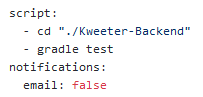
\includegraphics[width=0.33\textwidth]{images/TravisCIYml}
	\caption{TravisCI Yaml}
	\label{travisyml}
\end{figure}

Het bovenstaande script zorgt ervoor dat gradle tests automatisch worden uitgevoerd.
De uitslag van deze test is zichtbaar in het commit overzicht, zoals in \cref{fig:travisci-commits} te zien is.
Het TravisCI script wordt uitgelezen en uitgevoerd op een Ubuntu server van Travis, ontwikkelaars hebben hier zelf geen servers voor nodig.
De output van dit script kan ook uitgelezen worden op de website, dit zorgt ervoor dat je kan kijken hoe je tests draaien, en eventueel de oorzaak van errors kan vinden.

\section{Pull requests \& merging}
TravisCI draait je scripts automatisch bij elke commit die naar Github wordt gemaakt, en het resultaat is binnen een minuut zichtbaar.
Daarnaast kan een pull request worden tegengehouden zodra TravisCI een fout detecteerd in je build.
Als dit gebeurd moet de code eerst gerepareerd worden zodat de build weer werkt, daarna kan de pull request gemerged worden.